We need to tweak our model to make it perform at best. The PCA part was dealth with in a previous point and we found the optimal number of output dimensions to be around 80.\\
What is missing now is the backward-looking window for the Sharpe-Ratio used to rank strategies based on their performance. As mentioned before we will test the model in-sample with many different windows (short term ones ranging from 20 rading days up to 120 trading days).\\
The output is simply given by an analysis of performance in terms of Sharpe-Ratio and Sortino-Ratio for each window. A simple outlook is given by the following chart:

\begin{center}
	\centering
	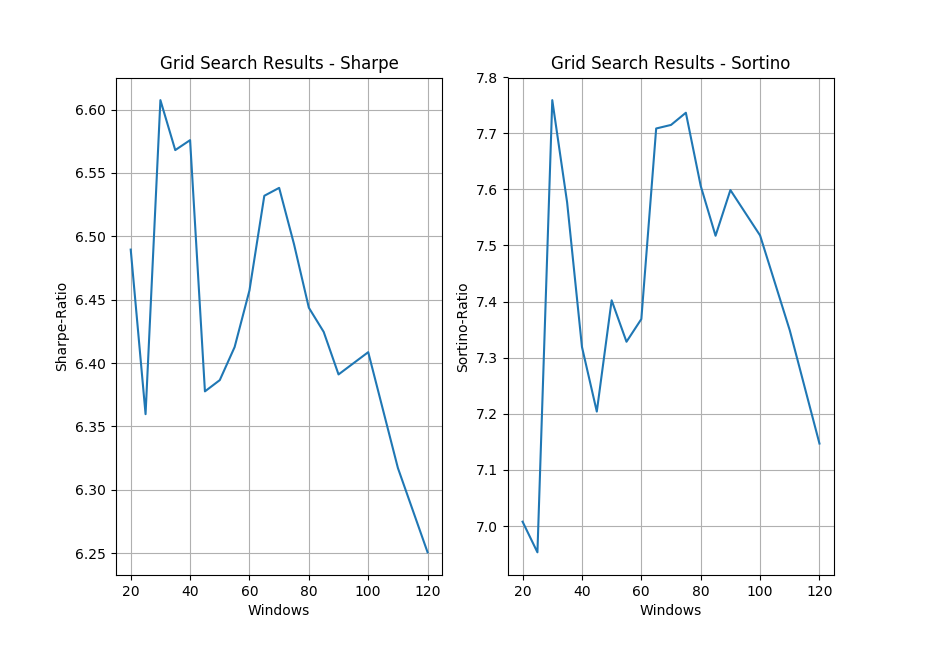
\includegraphics[width=0.7\textwidth]{HRP/CRP_Optimization.png}
	\captionof{figure}{GridSearch for the backward-looking period in the CRP method}
	\label{CRP_Optimization}
\end{center}

We can see how in-sample the optimal window seems to be in the 30 trading days area. This value is the best in both terms of Sharpe-Ratio and Sortino-Ratio therefore we have no doubts in sticking with it. Once this quick optimization has been run we are only missing the final results. To obtain these we simply run our algorithm on the whole out-of-sample period and we record the performance. The method is compared to a plain equally weighted portfolio and a dynamic minimum variance portfolio exposed in the Appendix. Let's explore the results:

\begin{center}
	\centering
	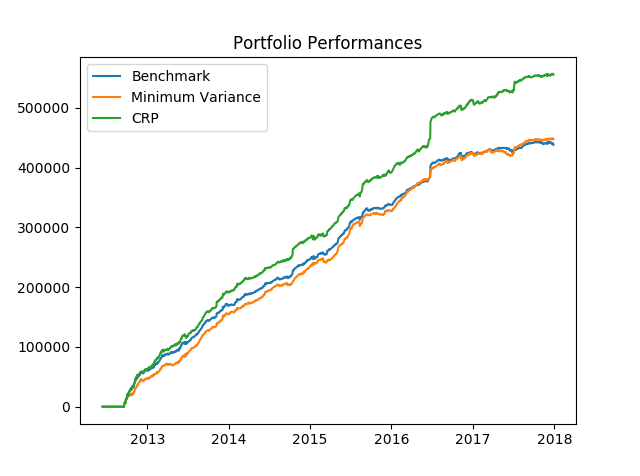
\includegraphics[width=0.6\textwidth]{HRP/OOS_Equity_Line.png}
	\captionof{figure}{Total Equity Line for the Clustered Risk Parity portfolio vs Benchmarks.}
	\label{CRP_Equity_LIne}
\end{center}

We can clearly and happily notice that the performance is definitely better than the benchmarks. The statistics for the three portfolios can be found in tables \ref{table:oos_perf_CRP} , \ref{table:oos_perf_benchmark_1}  and \ref{table:oos_perf_benchmark_2}  respectively.


\begin{table}
	\centering
	\begin{tabular}{c|c}
		\textbf{Statistic} & \textbf{Value} \\\hline
		Sharpe Ratio & 5.4977 \\ 
		Sortino Ratio & 7.707 \\ 
		Omega Ratio & 3.32 \\ 
		Skewness & 7.65 \\ 
		Kurtosis & 163.883 \\ 
		Maximum Drawdown (\% duration/duration) & 3.3 \\ 
		Longest Drawdown (days) & 48 \\ 
		Winning Days & 68.46 \\ 
	\end{tabular}
	%\label{table:oos_perf_CRP}
	\caption{\label{table:oos_perf_CRP} Performance Statistics for the out-of-sample period of the Clustered Risk Parity.}
\end{table}

\begin{table}
	\centering
	\begin{tabular}{c|c}
		\textbf{Statistic} & \textbf{Value} \\\hline
		Sharpe Ratio & 5.2342 \\ 
		Sortino Ratio & 7.6265 \\ 
		Omega Ratio & 3.06 \\ 
		Skewness & 4.66 \\ 
		Kurtosis & 89.54 \\ 
		Maximum Drawdown (\% duration/duration) & 3.5 \\ 
		Longest Drawdown (days) & 50 \\ 
		Winning Days & 70.942 \\ 
	\end{tabular}
	%\label{table:oos_perf_benchmark_1}
	\caption{\label{table:oos_perf_benchmark_1} Performance Statistics for the out-of-sample perid of the Equally Weighted Portfolio.}
\end{table}


\begin{table}
	\centering
	\begin{tabular}{c|c}
		\textbf{Statistic} & \textbf{Value} \\\hline
		Sharpe Ratio & 5.5309 \\ 
		Sortino Ratio & 7.1323 \\ 
		Omega Ratio & 3.09 \\ 
		Skewness & 1.2841 \\ 
		Kurtosis & 20.35 \\ 
		Maximum Drawdown (\% duration/duration) & 5.3 \\ 
		Longest Drawdown (days) & 77 \\ 
		Winning Days & 67.35 \\ 
	\end{tabular}
	%\label{table:oos_perf_benchmark_2}
	\caption{\label{table:oos_perf_benchmark_2} Performance Statistics for the out-of-sample period of the Minimum-Variance Portfolio.}
\end{table}

In this case we have achieved a good level of improvement if compared to the Genetic case. We really like that we had an improvement on most of our performance indicators. The improvement is not extremely huge, but seems to be statistically significant. I would claim we achieved a good level of diversification thanks to the Clustered risk-parity.